\documentclass[a4paper,12pt]{article}
\usepackage[T1]{fontenc}
\usepackage[utf8]{inputenc}
\usepackage[margin=1in]{geometry}
\usepackage{lmodern}
\usepackage{amssymb}
\usepackage{stmaryrd}
\usepackage{amsmath}
\usepackage{bbm}
\usepackage{graphicx}
\usepackage{url}
\usepackage[english]{babel}

\usepackage{hyperref}


\title{Parallel and Distrubuted Algorithms and Programs Project}
\author{Raphaël Monat}

\begin{document}

\maketitle

\tableofcontents

\section{Euler's approximation of differential equations}

\paragraph{Question 1a)}
Let's study $y' = ay$, with $a \in \mathbb{R}$. Using Euler's approximation, we get $y(t + dt) = y(t) + y'(t)dt = y(t) + a y(t) dt$, ie: $y(t + dt) = y(t) \cdot (1 + a \cdot dt)$. If we choose $a = -3$ and $dt = 1$, we have: $y(t+1) = - y(t)$. The solution to the differential equation is $y(t) = y(0) \cdot e^{-3x}$. The approximated solution is $y(k) = (-2)^{k+1}y(0)$ for any $k \in \mathbb{N}$. This is especially unacceptable, as even the asymptotic behavior is not the same.

\paragraph{Question 1b)} To compute the next step of an approximation of a differential equation of order n, we need to store the values of $u(t), ..., u^{(n-1)}(t)$, to be able to compute $u(t+dt)$: we need to store $n$ values.

\section{Cellular automata}

\paragraph{Question 2a)} We need to update every cell of the grid, so we need to call $\delta$ on each cell of this grid: $N \times M$ applications of $\delta$ to compute $X^t$ from $X^{t-1}$. To compute $X^t$ from $X^0$, we need $t \times NM$ applications of $\delta$.

\paragraph{Question 2b)} Suppose that we have a $p \times q$ 2D grid, and suppose also that $p \mid N$, $q \mid M$ for the sake of simplicity. Let $(i, j) \in \llbracket 0; p-1 \rrbracket \times \llbracket 0; q - 1 \rrbracket$. On the machine of coordinates $(i, j)$, we store the subgrid $\mathcal{G}_{i,j}$, of size $\frac{N}{p} \times \frac{M}{q}$, containing the following elements: $G_{k, l}$ with $(k, l) \in \llbracket i\frac{N}{p}; (i+1)\frac{N}{p}-1 \rrbracket \times \llbracket j\frac{M}{q}; (j+1)\frac{M}{q}-1 \rrbracket$. On each machine, we can localy update every element of the local grid, except the edges of the grid. To compute the edges of the grid, we need to get one edge of each grid $G_{i\pm1, j\pm1}$ (that is why we need communications). We will still compute the update of the edge cells on the local grid. We call the inner grid the local grid without the edges, and the outer edges of a grid, the edges it needs to receive from other processors to be able to update every edge cell. We can write the algorithm in the following way, which is executed on each subgrid:
\begin{enumerate}
\item For each cell in the inner local grid, compute the updated value of the cell, and put it in a temporary grid $T$. \textbf{In parallel} get the outer edges (except the four corners) of the neighbours $G_{i\pm1, j\pm1}$ (and send the edges of the local grid to the neighbours requesting it). 
\item For each cell (except the four corners) in the edges of the local grid, compute the updated value of the cell, and put it in the temporary grid. \textbf{In parallel} transmit the corners of a cell to the neighbor needing it (for example, if we are in (i, j) and receive from (i, j-1), we need to transmit to (i+1, j)), and receive the corners
\item Update the values of the corner.
\item Assign $T_{i,j}$ to $G_{i,j}$ (in fact, we can just use two grids, and update the good one using parity of the iteration number).
\end{enumerate}

\paragraph{Question 2c)}
Let $d$ be the cost of the application of $\delta$. We assume we have a 4-ports, full-duplex links. We analyse the cost of each step:
\begin{itemize}
\item Step 1: there are $\frac{(N-2)(M-2)}{pq}$ applications of $\delta$. In the meantime, we send/receive 2 rows and 2 columns of size $\frac{N}{p}$ and $\frac{M}{q}$ respectively. The cost of communications is $L + \max(\frac{N}{p}, \frac{M}{q}) \cdot b$. The cost of this step is $\max(d \cdot \frac{(N-1)(M-1)}{pq}, L + \max(\frac{N}{p}, \frac{M}{q}) \cdot b)$.
\item Step 2: there are $2 \cdot (\frac{N}{p} + \frac{M}{q})$ applications of $\delta$. In the meantime, we send/receive 4 elements, the communication cost is $L + b$. The cost is $\max(2d \cdot (frac{N}{p} + \frac{M}{q}), L + b)$
\item Step 3: there are $4$ applications of $\delta$.
\item We forget about step 4, as we can use two grids and never do any copy.
\end{itemize}
The cost is $$pq \cdot \left [ \max \left ( d \cdot \frac{(N-2)(M-2)}{pq}, L + \max(\frac{N}{p}, \frac{M}{q}) \cdot b \right )  + \max \left ( 2d \cdot (\frac{N}{p} + \frac{M}{q} \right ), L + b) + 4d \right ]$$ at each iteration of the computation.\\
The communications costs are $pq \cdot \left [ L + \max(\frac{N}{p}, \frac{M}{q}) + L + b \right ]$ in the 4-port model. The computation costs are $d \cdot NM$.

\paragraph{Question 2d)} This question has two answers, depending on which grid is considered:
\begin{itemize}
\item If the grid of the automaton is finite and bounded, there is a bit less communications, but this does not change anything in the 4-ports model.
\item If the grid of processors is bounded (it is necessarily finite...) (and if the grid of the automaton is still a torus), then the grid being on the edges should send at most two of their local automaton grid edges to the other edges. This would cost $q\cdot(L + \frac{N}{p}b) + p\cdot(L+frac{M}{q}b)$. The final communication costs are $$pq \cdot \left [ 2L + \max(\frac{N-2}{p}, \frac{M-2}{q}) + b + \max \left ( q\cdot(L + \frac{N}{p}b) + p\cdot(L+\frac{M}{q}b) \right ) \right ]$$
\end{itemize}


\section{Laplace operator and convolution}

\paragraph{Question 3a)} We consider the following cellular automaton: $\mathcal{A} = (2, \mathbb{R}^2, 1, \delta)$, with:

\begin{eqnarray*}
\delta : \left \{ \begin{array}{c c l }
  \mathbb{R}^2 & \longrightarrow & \mathbb{R}^2 \\
  u^{t}_{i,j}\ \pmb{,} \ u^{_{'} t}_{i,j} & \longmapsto & u^{t}_{i,j} + dt \cdot u^{_{'} t}_{i,j}\ \pmb{,} \ u^{_{'} t}_{i,j} + dt \cdot v^2 \cdot (u^t_{i+1,j} + u^t_{i-1, j} + u^t_{i, j+1} + u^t_{i, j-1} - 4 u^t_{i, j})\\
  \end{array} \right .
\end{eqnarray*}


\section{Performance evaluation}

\paragraph{Question 4a)} One simple porotocol to evaluate the scalability of my program is the following: pick a large enough example, and then use Simgrid to see how the communication costs evolve when augmenting the number of processors. However, Simgrid does not supports MPI IOs for now. It would have taken too much time to try to execute MPI programs over a lot of computers, that is why only present a plot with at most 8 processors.

\paragraph{Question 4b)} As usual, we see that at some point, there are too many processors, and the communications are then hindering the computations. Here, the number of CPUs is quite limited, because I cannot use Simgrid over a program using parallel I/Os. Below are the results using a 4-core/8-thread Intel Core i7 CPU, on $10^6$ iterations. The time is in seconds.

\begin{center}
  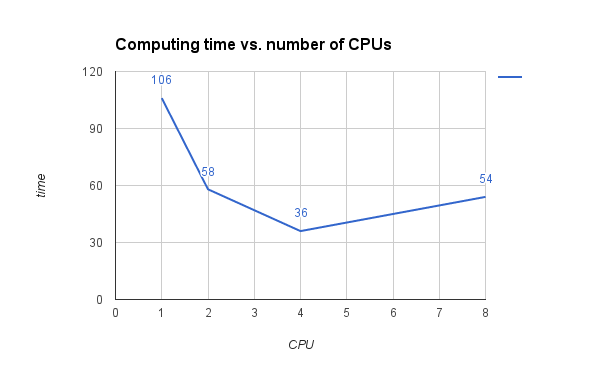
\includegraphics[scale=0.8]{results/perfs.png}
\end{center}


\section{Walls}

\paragraph{Question 5a)} We should transform $\mathcal{Q}$ into $\{0, 1\} \times \mathbb{R}^2$, to know if a cell is active or is a wall (0 meaning that the cell is a wall). We define two auxiliary functions f and f', and then update $\delta$: 


\begin{eqnarray*}
f : \left \{ \begin{array}{c c l }
  \mathcal{Q} & \longrightarrow & \mathbb{R} \\
  s \ \pmb{,} \ u\ \pmb{,} \ u' & \longmapsto & \mathbbm{1}_{\mathbb{N}^*}(s) \cdot u
  \end{array} \right .
\end{eqnarray*}


\begin{eqnarray*}
f' : \left \{ \begin{array}{c c l }
  \mathcal{Q} & \longrightarrow & \mathbb{R} \\
  s \ \pmb{,} \ u\ \pmb{,} \ u' & \longmapsto & \mathbbm{1}_{\mathbb{N}^*}(s) \cdot u'
  \end{array} \right .
\end{eqnarray*}


\begin{eqnarray*}
\delta : \left \{ \begin{array}{c c l }
  \mathcal{Q} & \longrightarrow & \mathcal{Q} \\
  x_{i,j}^t = (s \ \pmb{,} \ u^{t}_{i,j}\ \pmb{,} \ u^{_{'} t}_{i,j}) & \longmapsto &
  \begin{cases}s, 0, 0\mbox{ if s = 0}\\
    s, f(x^{t}_{i,j}) + dt \cdot f'(x^t_{i,j})\ \pmb{,} f'(x^t_{i,j}) + dt \cdot v^2 \cdot (f(x^t_{i+1,j}) \\+ f(x^t_{i-1, j}) + f(x^t_{i, j+1}) + f(x^t_{i, j-1}) - 4 f(x^t_{i, j})) 
    \end{cases}\\
  \end{array} \right .
\end{eqnarray*}

\section{Sensors}

\paragraph{Question 6a)} We suppose that sensors are never walls (it would not be interesting at all, as the record variable would always be 0). We also suppose that we record only $u_{i,j}^2$ and not $q^2$ for some $q \in \mathcal{Q}$. So, we just need to change $\mathcal{Q}$ into $\{0,1,2\} \times \mathbb{R}^2 \times \mathbb{R}$, where 0 means a wall, 1 means a normal cell, and 2 means a sensor. We need to update $\delta$:

\begin{eqnarray*}
\delta : \left \{ \begin{array}{c c l }
  \mathcal{Q} & \longrightarrow & \mathcal{Q} \\
  x_{i,j}^t = (s \ \pmb{,} \ u^{t}_{i,j}\ \pmb{,} \ u^{_{'} t}_{i,j} \ \pmb{,} \ c) & \longmapsto &
  \begin{cases}s, 0, 0\mbox{ if s = 0}\\
    s, f(x^{t}_{i,j}) + dt \cdot f'(x^t_{i,j})\ \pmb{,} f'(x^t_{i,j}) + dt \cdot v^2 \cdot (f(x^t_{i+1,j}) \\+ f(x^t_{i-1, j}) + f(x^t_{i, j+1}) + f(x^t_{i, j-1}) - 4 f(x^t_{i, j})),\\
    \begin{cases} 0 \mbox{ if }s \leq 1\\
      c + (f(x^{t}_{i,j}) + dt \cdot f'(x^t_{i,j}))^2 \mbox{ if s = 2} \\
    \end{cases}
  \end{cases}
  \end{array} \right .
\end{eqnarray*}


\section{Local environment characteristics}

\paragraph{Question 7a)} We need to change $\mathcal{Q}$ into $\{0,1,2\} \times \mathbb{R}^2 \times \mathbb{R} \times \mathbb{R}$, the last argument being the local speed. In $\delta$, we just update $v$ into $v_{i,j}$.

\paragraph{Question 7c)} We need to change a bit our implementation, but nothing really important. 

\section{Experimental Science}

\paragraph{Question 8a)} We need to check if this is close to reality or not. We could try to see if the propagation is correct, and then try to observe more complex phenomena, like interferences. Propagations look realistic if the time interval $dt$ is small enough (see results/sample\_type1\_*.mp4). Concerning interferences, I implemented a program generating something roughly like Young's experiment. Interferences are quite realistic, see the results/young.mp4 file for example.

\section{Notes on the implementation}

I have 3 different implementations: one concerning step 0, one concerning steps 1, 2 and 3 and one concerning step 4. Although step123.c and step4.c are really similar, I prefered to create distinct files. I could have structured a lot more the code, but a lot of functions would have had too much arguments for this basic project. In steps 1 and higher, all the I/Os are done in parallel using MPI functions, except the output of sensor values. It would have been quite difficult and not that interesting to handle the cases where we do not have $p \mid N$ and $q \mid M$, so they are not supported (in particular, MPI\_Type\_create\_subarray forces the divisibility condition). I also added a new parameter called frequency, to store only one part of all the dump files (thus reducing the writing time, and the time to generate the video). One last remark: sensor values in the file are not sorted by any order, as it was not asked in the subject.
\par Please try \textit{make demo}.

\end{document}
